%%%%%%%%%%%%%%%%%%%%%%%%%%%%%%%%%%%%%%%%%%%%%%%%%%%%%%%%%%%%%%%%%%%%%
%%                                                                 %%
%% Please do not use \input{...} to include other tex files.       %%
%% Submit your LaTeX manuscript as one .tex document.              %%
%%                                                                 %%
%% All additional figures and files should be attached             %%
%% separately and not embedded in the \TeX\ document itself.       %%
%%                                                                 %%
%%%%%%%%%%%%%%%%%%%%%%%%%%%%%%%%%%%%%%%%%%%%%%%%%%%%%%%%%%%%%%%%%%%%%
\RequirePackage{tikz}

\documentclass[pdflatex,referee,iicol,sn-basic]{sn-jnl}

%%%% Standard Packages
\usepackage{xcolor,hyperref}
\usepackage[autostyle=false, style=english]{csquotes}
%%%%

% Avoid having to ``quote'' verbosely (csquotes package)
\MakeOuterQuote{"}

% Make Orcid icon
\definecolor{lime}{HTML}{A6CE39}
\DeclareRobustCommand{\orcidicon}{%
	
\begin{tikzpicture}
	\draw[lime, fill=lime] (0,0) 
	circle [radius=0.16] 
	node[white] {{\fontfamily{qag}\selectfont \tiny ID}};
	\draw[white, fill=white] (-0.0625,0.095) 
	circle [radius=0.007];
	\end{tikzpicture}
	\hspace{-2mm}
}

\foreach \x in {A, ..., Z}{%
	\expandafter\xdef\csname orcid\x\endcsname{\noexpand\href{https://orcid.org/\csname orcidauthor\x\endcsname}{\noexpand\orcidicon}}
}

% Define the ORCID iD command for each author separately.
\newcommand{\orcidauthorA}{0000-0002-3420-4576}
\newcommand{\orcidauthorB}{0000-0001-9402-0851}

% Shorter italic dev/msc/std
\newcommand{\dev}{\textit{dev}}
\newcommand{\msc}{\textit{msc}}
\newcommand{\std}{\textit{std}}

%%%%%=============================================================================%%%%
%%%%  Remarks: This template is provided to aid authors with the preparation
%%%%  of original research articles intended for submission to journals published 
%%%%  by Springer Nature. The guidance has been prepared in partnership with 
%%%%  production teams to conform to Springer Nature technical requirements. 
%%%%  Editorial and presentation requirements differ among journal portfolios and 
%%%%  research disciplines. You may find sections in this template are irrelevant 
%%%%  to your work and are empowered to omit any such section if allowed by the 
%%%%  journal you intend to submit to. The submission guidelines and policies 
%%%%  of the journal take precedence. A detailed User Manual is available in the 
%%%%  template package for technical guidance.
%%%%%=============================================================================%%%%

\jyear{2021}%

%% as per the requirement new theorem styles can be included as shown below
\theoremstyle{thmstyleone}%
\newtheorem{theorem}{Theorem}%  meant for continuous numbers
%%\newtheorem{theorem}{Theorem}[section]% meant for sectionwise numbers
%% optional argument [theorem] produces theorem numbering sequence instead of independent numbers for Proposition
\newtheorem{proposition}[theorem]{Proposition}% 
%%\newtheorem{proposition}{Proposition}% to get separate numbers for theorem and proposition etc.

\theoremstyle{thmstyletwo}%
\newtheorem{example}{Example}%
\newtheorem{remark}{Remark}%

\theoremstyle{thmstylethree}%
\newtheorem{definition}{Definition}%

\raggedbottom
%%\unnumbered% uncomment this for unnumbered level heads

\begin{document}

\title{Short-term neuronal and synaptic plasticity act in synergy for deviance detection in spiking networks}

%%=============================================================%%
%% Prefix	-> \pfx{Dr}
%% GivenName	-> \fnm{Joergen W.}
%% Particle	-> \spfx{van der} -> surname prefix
%% FamilyName	-> \sur{Ploeg}
%% Suffix	-> \sfx{IV}
%% NatureName	-> \tanm{Poet Laureate} -> Title after name
%% Degrees	-> \dgr{MSc, PhD}
%% \author*[1,2]{\pfx{Dr} \fnm{Joergen W.} \spfx{van der} \sur{Ploeg} \sfx{IV} \tanm{Poet Laureate} 
%%                 \dgr{MSc, PhD}}\email{iauthor@gmail.com}
%%=============================================================%%

\author[1]{\fnm{Felix Benjamin} \sur{Kern} \orcidA{}}\email{kernfel@gmail.com}

\author*[1]{\fnm{Zenas C.} \sur{Chao} \orcidB{}}\email{zenas.c.chao@gmail.com}

\affil[1]{\orgdiv{International Research Center for Neurointelligence (WPI-IRCN)}, \orgname{The University of Tokyo}, \orgaddress{\city{Tokyo}, \country{Japan}}}

%%==================================%%
%% sample for unstructured abstract %%
%%==================================%%

\abstract{TODO}


\keywords{keyword1, Keyword2, Keyword3, Keyword4}

\maketitle

\section{Introduction}\label{sec-intro}


\section{Methods}\label{sec-methods}

\subsection{Model}\label{sec-model}

We modeled neurons as leaky integrate-and-fire units whose membrane potential $V_m$ at time $t$ followed
\begin{equation}
    \tau_m \frac{dV_m}{dt} = (V_{rest}-V_m) + I_{syn}(t)
\end{equation}
with $tau_m = 30$~ms the membrane time constant and $V_{rest} = -60$~mV the resting membrane potential. Synaptic currents were modeled in a conductance-based manner, following
\begin{equation}
    I_{syn} = g_e(E_e-V_m) + g_i(E_i-V_m)
\end{equation}
with $E_e = 0$~mV and $E_i = -100$~mV the excitatory and inhibitory reversal potentials, respectively. Synaptic conductances evolved according to
\begin{align} 
    \tau_e \frac{dg_e}{dt} &= -g_e + \sum_{j \in \boldsymbol E} U x_j w \delta(t - \hat{t_j}) \nonumber \\
    \tau_i \frac{dg_i}{dt} &= -g_i + \sum_{j \in \boldsymbol I} w \delta(t - \hat{t_j}) \label{eqn-gsyn}
\end{align}
with $\tau_e = 2$~ms the excitatory time constant, echoing AMPA receptor dynamics \citep{Hausser1997-cn}, $\tau_i = 4$~ms the inhibitory time constant, echoing GABA-A receptor dynamics \citep{Destexhe1994-oc}, $\boldsymbol E$ and $\boldsymbol I$ the sets of presynaptic excitatory and inhibitory neurons, respectively, $w$ the synaptic weight, $\delta(\cdot)$ the Dirac delta function, and $\hat{t}$ the spike times.

Excitatory, but not inhibitory, synapses were subject to short-term depression (STD), simplified from \cite{Tsodyks1997-qt}; since synaptic transmission was not stochastic, we modeled the depression variable $x_j$ as a property of the presynaptic neuron $j$,
\begin{equation}
    \tau_x \frac{dx_j}{dt} = (1-x_j) - U x_j \delta(t - \hat{t}) \label{eqn-xsyn}
\end{equation}
with recovery time constant $\tau_x = 150$~ms and release fraction $U = 0.4$.

When a neuron's membrane potential reached the firing threshold $V_\theta$, a spike was emitted, and the potential was clamped to $V_m = V_{reset} = -74$~mV for a fixed refractory period of 3~ms (excitatory neurons). Inhibitory neurons were modeled as fast-spiking cells with a refractory period of 2~ms and a constant firing threshold $V_\theta = \theta_0 = -54$~mV \citep{Mensi2012-au}. In contrast, excitatory neurons were modeled with threshold adaptation (TA) as in \cite{Teeter2018-iz}, following
\begin{align}
    V_\theta &= \theta_0 + \theta(t) \nonumber \\
    \tau_{\theta} \frac{d\theta}{dt} &= -\theta + \hat{\theta} \delta(t - \hat{t}) \label{eqn-TA}
\end{align}
with increment $\hat{\theta} = 1$~mV and decay time constant $\tau_{\theta} = 1$~s \citep{Pozzorini2015-ei}.

\begin{figure*}%
    \centering
    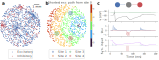
\includegraphics{fig1.pdf}
    \caption{}
    \label{fig1}
\end{figure*}
\textbf{Fig. 1} Model and paradigm. \textbf{a} Membrane and synaptic dynamics of a neuron innervated by an excitatory and an inhibitory neuron firing pre-determined spikes, illustrated above the plots. The excitatory connection has weight $w = 3$ for demonstration purposes only; a single connection with $w = 1$ is normally unable to evoke postsynaptic firing. Top: Inputs to the (post-)synaptic conductances $g_e$ and $g_i$ (vertical bars), and the STD depression variable $x_{Exc}$ of the excitatory presynaptic neuron (dashed line). Note that excitatory inputs are equal to $U x_{Exc} w$ as per Equation \ref{eqn-gsyn}. Middle: Excitatory and inhibitory synaptic conductances ($g_e$ and $g_i$, respectively). Bottom: Membrane voltage, firing threshold baseline (gray) and adaptive threshold, demonstrating TA in the excitatory postsynaptic neuron. \textbf{b} Sample network layout, showing the spatial location of excitatory and inhibitory neurons, and all outgoing synaptic connections from two neurons of each type. \textbf{c} Distance from stimulation site 1 in terms of minimum number of excitatory synapses. Stimulation is provided to the 10 neurons nearest to the center of each of 5 stimulation sites (large circles), which are regularly spaced on a circle with a radius of 2.5 mm. \textbf{d} Illustration of the stimulation paradigm. Each marker represents a stimulation, with the stimulus identity indicated by color. The target stimulus (A) is represented as solid red, and non-target stimuli are represented with faded colors. Three randomized sequences were presented, containing 80\% A and 20\% B (\std{}), 20\% A and 80\% B (\dev{}), and 20\% of each of 5 stimuli, including A and B (\msc{}). Note that, while the onset asynchrony of 500 ms is represented faithfully, the horizontal extent of the stimulation markers has no meaning; stimuli were presented instantaneously rather than over an extended period.

Figure \ref{fig1}a shows the internal and presynaptic dynamics of an excitatory neuron in a contrived example for the purpose of illustration. The model was implemented in Brian2 \citep{Stimberg2019-tc}, accelerated with Brian2GeNN \citep{Stimberg2020-go}, and simulated with an integration time step of 1~ms. Synaptic delay was not modeled explicitly, but spikes were delivered, and voltages reset, in the time step following spike emission. We simulated neurons without any stochasticity in either their inputs or their parameters, other than network structure (described below), in order to ensure that our results were driven purely by the experimental paradigm, rather than any model-internal sources of noise.

800 excitatory and 200 inhibitory neurons were placed randomly in a two-dimensional circular space with a radius of 4~mm, and formed synapses of weight $w = 1$ with 50 randomly selected postsynaptic partners within a range of 2~mm (excitatory) or 1~mm (inhibitory), reflecting the notion that excitatory neurons project over longer distances, while inhibitory neurons mainly connect to their local neighborhood. Connectivity and weights remained fixed throughout. Stimulation sites were evenly distributed 2.5~mm from the center of the dish, and stimulation delivered a one-time increase in $g_e$ to the 10 closest neurons, sufficient to trigger 2-3 spikes each. Figure \ref{fig1}b shows a representative example of the resulting network structure. In Figure \ref{fig1}c, we show the distance from the neurons stimulated at site 1 to each neuron in this network, in terms of the minimum number of excitatory synapses that need to be traversed to reach the target, in order to give an intuition for how activity may spread. Networks were pseudo-randomly generated according to the above scheme and screened for minimal stimulus response: Networks where fewer than 500 neurons responded to stimulation at any of the five sites after full recovery were discarded. In total, 30 networks were used for the experiments described below.

\subsection{Paradigm}\label{sec-paradigm}

To investigate deviance detection, we used a classical oddball paradigm as illustrated in Figure \ref{fig1}d, presenting a total of 500 stimuli at regular intervals of 500~ms. Target stimuli (labeled "A" or "target" hereafter) and distractor stimuli (labeled B to E) were presented in three randomized sequences: The "standard" sequence (\std{}), consisting of 400 presentations of A and 100 presentations of B; the "deviant" sequence (\dev{}) with 100 A and 400 B, and the many-standards control sequence (\msc{}) with 100 presentations of each of the stimuli A through E. In this way, A is presented as the predominant and therefore expected stimulus (\std{}), as an infrequent violation of an expectation (of B, \dev{}), and, to control for pure adaptation effects, as an equally infrequent stimulus with no strong expectation of any particular input (\msc{}).

In each network, we simulated oddball sequences with two A/B stimulus pairs (sites 1 and 2 in one pair, and sites 3 and 5 in the other pair), where each stimulus site in a pair was used once as target (A) and once as non-target (B), and a single \msc{} sequence involving all sites. Networks were reset to a fully recovered state between sequence presentations to guarantee their independence. This yielded 4 complete data sets per network, or a total of 120 data sets across all networks.

In order to disentangle the effects of STD and TA, we ran all simulations in four conditions: Without any short-term plasticity, with either TA only or STD only, and with both STD and TA (labeled STD+TA in the following, and corresponding to the full model as described above). To turn off STD, we replaced Equation \ref{eqn-xsyn} with a constant $x = 1$, but retained the scaling of inputs to $g_e$ with $U$ in Equation \ref{eqn-gsyn}. This corresponds to immediate recovery ($\tau_x = 0$) and was done to maintain the magnitude of the excitatory postsynaptic potential (EPSP) in the recovered state regardless of whether STD was turned on or off. To turn off TA, we replaced Equation \ref{eqn-TA} with a constant $V_{\theta} = \theta_0$, making the firing threshold completely unadaptive.

\subsection{Sample network}\label{sec-sample}

We present most of our analysis at two levels: We first detail the processes leading to deviance detection on a sample network, then confirm the highlighted trends statistically with reference to the full set of 120 networks and stimulus assignments. The sample network was chosen to be roughly representative of the population as follows: We assessed each network's average response to stimulation with A and B in the \msc{} sequence and calculated z-scores with respect to the population. We considered only networks whose absolute z-score was less than 1 for both A and B responses, then hand-picked a sample network and stimulus assignment that exhibited both an increased deviance detection index (see Equation \ref{eqn-ddi} below) in STD+TA over TA only, and greater \msc{} than \std{} responses in both STD+TA and TA only conditions.

\section{Results}\label{sec-results}

\subsection{Deviance detection}\label{sec-dd}

We define deviance detection as a network's ability to pick out unexpected inputs from an otherwise homogeneous or otherwise unsurprising stream of inputs. Following related research \citep{Kubota2021-dx,Harms2014-ah,Jacobsen2001-sc}, we were careful to exclude effects due to stimulus identity (i.e., avoiding direct comparisons between different stimuli) or due to adaptation to frequent stimulus presentation (i.e., avoiding direct comparisons of A in the \dev{} sequence to A in the \std{} sequence). In other words, we used the \msc{} sequence as a neutral baseline where the target stimulus was presented no more often than in the \dev{} sequence, but no expectation of a competing stimulus B could be formed. To quantify deviance detection, we compared the mean number of spikes fired per neuron in response to target stimulus A in the \dev{} and \msc{} sequences, denoted as $R^A_{dev}$ and $R^A_{msc}$, defining a deviance detection index (DDI) as
\begin{equation}
    DDI = \frac{R^A_{dev} - R^A_{msc}}{R^A_{dev} + R^A_{msc}} \label{eqn-ddi}
\end{equation}

\begin{figure*}%
    \centering
    \includegraphics{fig2.pdf}
    \caption{}
    \label{fig2}
\end{figure*}
\textbf{Fig. 2} Deviance detection in our model. \textbf{a} Sample network target response intensity by trial type. Each horizontal line of the plot summarizes the network response in one target trial in terms of spikes per integration time step. Target trials are taken from the \std{} (400), \msc{} (100), and \dev{} (100) sequences, and sorted by sequence time (earliest trials are at the bottom of each section). \textbf{b} Response summary, showing average network-wide spike counts in target trials in each sequence. The underlying data are the same as in panel a. Note how the \dev{} response is very large, followed by an intermediate \msc{} response and a low \std{} response.
\textbf{c} Response sizes $R^A_{dev}$ and $R^A_{std}$, normalized by $R^A_{msc}$, across networks and stimuli (n = 120). In this and later boxplots, the median is indicated with an orange line, notches indicate the 95\% confidence interval for the median calculated by bootstrap with 10000 iterations, boxes indicate the inter-quartile range (IQR), whiskers extend to 1.5 times the IQR or to the data extrema, whichever is less, and fliers indicate individual data points beyond the whisker end points.
\textbf{d} Deviance detection indices (DDI, see Equation {eqn-ddi}) across networks and stimuli

To show that our model is capable of deviance detection, we first show the responses of the sample network in all sequences (\dev{}, \msc{}, and \std{}) in Figure \ref{fig2}a. Here, each row corresponds to one trial, aligned to stimulus input at t = 0, with the number of spikes in each millisecond bin indicated by color. All responses share an early activity pattern, which derives from the stimulated neurons and their immediate postsynaptic targets, but differences soon start to emerge. The \dev{} sequence responses, shown at the top of the plot, exhibit a clear peak in activity around 15 ms after stimulation. The \std{} sequence responses show a later, more diffuse activity peak around 20 ms, and the \msc{} sequence responses lack any obvious activity cluster. We sum these patterns up in Figure \ref{fig2}b, where we show the mean network activity, in terms of spikes per millisecond bin, across trials of each type. Clearly, the target response in the \dev{} sequence is greater than either the \msc{} or the \std{} response.

We could readily identify similar patterns emerging across most networks and stimulus assignments. To show that deviance detection is robust to network and stimulus identity, we calculated the average spike count per neuron per target trial for each network and stimulus assignment, and compared these across sequences. Figure \ref{fig2}c shows a summary of the average \dev{} and \std{} response sizes, normalized by the response in the \msc{} sequence. The data clearly confirmed that \dev{} responses were larger than \msc{} (T = 6.38e+03, p = 2.75e-13; one-sided Wilcoxon signed-rank test, n = 120), and \std{} responses smaller (T = 687, p = 6.42e-15). Accordingly, the DDI (Figure \ref{fig2}d) was positive in most networks (T = 5.97e+03, p = 4.75e-10, median 0.114). This shows that our model was well behaved and suitable for an investigation of deviance detection.

\begin{figure*}%
    \centering
    \includegraphics{fig3.pdf}
    \caption{}
    \label{fig3}
\end{figure*}
\textbf{Fig. 3} Deviance detection under model ablation. \textbf{a} Sample network responses to target stimulation, with the deviance detection index in each instance noted in the plot titles. Lines show the average (trial mean +- SEM, left axis) network-wide spike counts in target trials in each sequence. Boxes summarize the spike count totals per trial (right axis), the means of which form the basis for index calculations (see panel c). Note the different axis scaling on the top row (without TA) and the bottom row (with TA). \textbf{b} Deviance detection indices across networks and stimuli. Asterisks indicate data greater than 0, established with a Wilcoxon signed-rank test at a significance level 0.05. See main text for detailed statistics

Having confirmed the presence of deviance detection in our model, we turned to an ablation approach to try to identify how the two short-term plasticity mechanisms in the model, STD and TA, enabled the networks to learn relevant regularities. Figure \ref{fig3}a shows the responses to target stimulation of the sample network under ablation. With no plasticity, the responses are indistinguishable between sequences, yielding a DDI of 0, and indicating that stimulation did not have any long-lasting effects in membrane voltage or synaptic conductance. With STD only, the response in the \dev{} sequence developed earlier and very slightly larger, yielding a DDI of 0.03. With TA only, the response became noticeably smaller, but the sequences became readily distinguishable, with high \dev{}, intermediate \msc{}, and low \std{} responses, yielding a DDI of 0.19. Finally, in the full model, the \dev{} response stood out more clearly, leaving much smaller \msc{} and \std{} responses and yielding a DDI of 0.4.

Finally, across networks and stimuli, the DDI (Figure \ref{fig3}c) was exactly 0 as expected in the ablation with no plasticity, not significantly different from 0 with STD only (T = 3.2e+03, p = 0.262, median -2.1e-04; two-sided Wilcoxon, n = 120), but clearly positive for TA only (T = 5.85e+03, p = 3.1e-09, median 0.077; one-sided Wilcoxon, n = 120) and the full model (T = 5.97e+03, p = 4.75e-10, median 0.114). To our surprise, the DDI of the full model was significantly greater than that of either plasticity mechanism alone (STD: T = 6.1e+03, p = 4.95e-11; TA: T = 4.87e+03, p = 0.000604), and greater too than the sum of the DDI values across both STD only and TA only models (T = 5.12e+03, p = 4.52e-05). This suggests that TA and STD act not as independent mechanisms in this paradigm, but rather interact constructively to enhance the network's ability to encode input regularities.

In the following, we will first build an understanding of how TA leads to deviance detection when acting alone, i.e. in the ablated TA only model, working backwards from the increased target response in \dev{}, identifying and tracing causal factors step by step. Then, we will build on this understanding to elucidate how the addition of STD, which was shown above to be ineffective for deviance detection on its own, can lead to an increased deviant response in the full model.

\subsection{The role of TA in deviance detection}\label{sec-ta}

To understand why the same stimulus A evoked a higher response in \dev{} than in \msc{} with TA only, we first compared the average responses in the two sequences, sorting neurons by their response onset to permit a high-resolution view of the stimulus response as it propagates through the network. As shown in Figure \ref{fig4}a (left and middle), we found that the response developed in a qualitatively similar fashion in both sequences. The contrast (right) revealed a clear increase in \dev{} spikes, particularly in the later parts of the response, as shown by the predominance of orange areas, indicating higher \dev{} activity. Since the stimulus was identical in both sequences, and TA was the only plasticity mechanism in play, these differences had to be due to (1) different firing thresholds, and/or (2) different synaptic currents as a consequence of different prior activity within the trial.

\begin{figure*}%
    \centering
    \includegraphics{fig4.pdf}
    \caption{}
    \label{fig4}
\end{figure*}
\textbf{Fig. 4} Responses to \dev{} target trials are larger due to lower $\theta$.
\textbf{a} Target trial average post-stimulus spike histogram in the sample network, showing trial time along the horizontal axis, and neurons along the vertical, sorted by the time of the first recorded spike across all trials and sequences. Left and middle column, target trials in \dev{} sequence and \msc{} sequence, respectively; right column, contrast between these two.
\textbf{b} Target trial average of the threshold adaptation voltage $\theta$, with neuron order and columns as in panel a.
\textbf{c} Target trial average of the membrane potential $V_m$, with neuron order and columns as in panel a. The first 10 ms of the neurons under direct stimulation are masked out to avoid saturation of the colormap.
\textbf{d} Relationship across excitatory neurons of the sample network between the contrast (\dev{} - \msc{}) in $\theta$ at the start of target trials and the contrast in average number of spikes fired in target trials, and associated linear regression.
\textbf{e} Network-wide median contrast (\dev{} - \msc{}) in $\theta$ across networks and stimuli, plotted against the Pearson correlation coefficients $\rho$ of the relationship shown in the previous panel ($\Delta \theta$ vs response size contrast across excitatory neurons). Each marker corresponds to one network and target stimulus. Red markers indicate a significant negative correlation (two-sided Wald test, significance level 0.05). Inset histograms show the distribution of the corresponding values, with orange portions indicating the 95\% confidence interval of the median, calculated by bootstrap with 10000 iterations.
\textbf{f} In the sample network, contribution of the contrast in $\theta$ and $V_m$ to bins with increased firing in \dev{} (i.e., positive/red bins in the spike probability contrast, panel a), weighted by that same contrast.
\textbf{g} Contribution of $\theta$ relative to the sum of the absolute values of the weighted contributions in panel f.
\textbf{h} Relative contribution of $\theta$ across networks and stimuli, showing median (solid line) and inter-quartile range (shaded area)

We quantified the former with the strength of adaptation $\theta$ (Equation \ref{eqn-TA}), i.e., the amount by which the firing threshold was raised due to TA. As shown in Figure \ref{fig4}b, there was a clear and widespread lowering of thresholds at the start of target \dev{} trials relative to \msc{}, visible both in the raw data (left and middle panels) and in the contrast (right panel, early blue portions). On the other hand, once the bulk of activity had occurred, many neurons showed higher thresholds in \dev{} (right panel, later orange portions), since they spiked more often. Finally, note that inhibitory neurons, which were modeled without TA, naturally showed no difference in $\theta$, leading to numerous horizontal breaks in the plot.

To assess the difference in synaptic currents in a way that allowed direct comparison to $\theta$, we referred to the membrane voltage $V_m$, which is largely independent from and complementary to the firing threshold, and driven mostly by presynaptic inputs, resets after spikes notwithstanding. As the immediate cause of neuronal spiking, the overall pattern of $V_m$ (Figure \ref{fig4}c) largely reflected that seen in spiking activity. The contrast (right panel) shows not only a notable relative increase in membrane voltages in \dev{} around the typical response time (note the orange band running along the response front), but also an increased hyperpolarization starting immediately after due to post-spike resets.

Based on these measures, we then asked why there were more spikes in \dev{} trials. We first focused on the contribution of $\theta$ alone in an effort to confirm that thresholds are lower in \dev{}, and that this reduction in thresholds causes increased firing. We correlated the contrast (dev - msc) of $\theta$ at the start of target trials (i.e., at the left edge of the contrast histogram in Figure \ref{fig4}b) with the target trial response size contrast, across excitatory neurons. In the sample network (Figure \ref{fig4}d), we found that thresholds were clearly lower in \dev{} than \msc{} (T = 2.69e+04, p = 1.58e-92, median = -0.166 mV; one-sided Wilcoxon, n = 800 excitatory neurons), and that this decrease was accompanied by an increase in the target trial response at the level of individual neurons (Pearson's $\rho$ = -0.424, p = 1.6e-36; one-sided Wald test, n = 800). As shown in Figure \ref{fig4}e, this relationship held across networks and stimuli: The median $\theta$ among excitatory neurons was lower in \dev{} than \msc{} (T = 514, p = 1.67e-16, grand median = -0.094 mV; one-sided Wilcoxon, n = 120), indicating that networks were less adapted during oddball sequences. In addition, the neuron-level correlation between the contrasts in $\theta$ and target response was almost universally negative (T = 40, p = 2.68e-21, median = -0.357). This indicates that neurons with a greater decrease in $\theta$ in \dev{} tended to respond more strongly to target stimuli.

Yet, as we saw in Figure \ref{fig4}c, the membrane voltages also differed between the two sequences. In order to assess the relative contribution of $\theta$ to the increased \dev{} response, we chose to focus exclusively on time points with higher firing probability in the \dev{} sequence, discarding data points with equal or lower firing probability relative to the \msc{} sequence. We then weighted the remaining contrasts in $\theta$ and $V_m$ by the magnitude of the response difference, and summed across neurons. The resulting time courses, shown in Figure \ref{fig4}f, show how much these two measures contributed to the increased \dev{} response. While thresholds were slightly lowered throughout the response, the membrane potential was dramatically increased. In relative terms (Figure \ref{fig4}g), $\theta$ constituted a major driver of increased firing right at the onset of the response, as well as briefly towards the end of the response. A similar pattern emerged across networks and stimuli, as shown in Figure \ref{fig4}h. Here, only the initial response was driven mainly by $\theta$, while later differences were largely explained by differences in $V_m$, leading to a relative TA contribution of less than 20\% on average. This indicates that adaptation initiated and dominated the increase in firing at the start of trials, whereas the late response was enlarged primarily as a result of increased presynaptic excitation.

Having established that the increased response to A in \dev{} trials was driven by lower thresholds before stimulation, we next turned to the cause of this reduction. A priori, since threshold adaptation is a direct reflection of activity, and since the response to target trials was larger in \dev{} than in \msc{}, the lower thresholds in \dev{} must have been caused by lower activity in non-target trials, i.e. lower responses to B in \dev{} than to B through E in \msc{}. Yet, since activity is modulated by thresholds as shown above, and since the dev sequence was random, meaning that thresholds before stimulation could carry no information about the upcoming stimulus, we might expect the lowered thresholds in \dev{} to yield not only higher target responses, but also higher non-target responses. To resolve this apparent paradox, we will turn to an analysis of the spatial arrangement of activity and adaptation.

\begin{figure*}%
    \centering
    \includegraphics{fig5.pdf}
    \caption{}
    \label{fig5}
\end{figure*}
\textbf{Fig. 5} Lower $\theta$ in \dev{} is a consequence of lower \dev{} non-target response magnitude.
\textbf{a} $\theta$ at the start of A trials (mean over trials) in the sample network, with each neuron shown in its spatial location. Left and middle column, raw averages for \dev{} and \msc{} sequences, respectively; right column, contrast between \dev{} and \msc{} averages. A and B stimulus locations for this and following figures are highlighted in the left plot; see Figure \ref{fig1} for the locations of the remaining stimuli used in the \msc{} sequence.
\textbf{b} Average response (in spikes per trial) to non-target trials (B in \dev{}, B, C, D, and E in \msc{}). Columns are arranged as in panel a.
\textbf{c} Relationship across excitatory neurons of the sample network between the contrast (\dev{} - \msc{}) in average number of spikes fired in response to non-target stimulation and the contrast in $\theta$ at the start of target trials, and associated linear regression.
\textbf{d} Network-wide median contrast (\dev{} - \msc{}) in the non-target response magnitude across networks and stimuli, plotted against the Pearson correlation coefficients $\rho$ of the relationship shown in the previous panel (non-target response size contrast vs $\Delta \theta$ across excitatory neurons). Each marker corresponds to one network and target stimulus. Red markers indicate a significant positive correlation (one-sided Wald test, significance level 0.05). Inset histograms show the distribution of the corresponding values, with orange portions indicating the 95\% confidence interval of the median, calculated by bootstrap with 10000 iterations

First, we mapped the average value of $\theta$ at the start of target trials to the spatial location of the neurons, as shown in Figure \ref{fig5}a. In the \msc{} sequence, $\theta$ was roughly evenly distributed across the network, consistent with the random, distributed nature of stimulation. Conversely, in the \dev{} sequence, neurons near the non-target stimulation site (B) were strongly adapted, whereas the majority of the network was less adapted, consistent with the data shown above.

Next, we turned to the likely cause of this difference, the non-target responses (Figure \ref{fig5}b), mapped into space as the average number of spikes fired in each neuron. As expected, the pattern of activity in non-target trials, constituting 80\% of all trials, closely matched that of the thresholds. Notably, although the comparison is between 400 B trials in \dev{}, and only 100 B trials (alongside the same number of C, D and E trials) in \msc{}, only a small handful of neurons responded more to non-target stimulation in \dev{}, most of these very close to the stimulation site of B.

Correlating the non-target response contrast (\dev{} - \msc{}) with the contrast in $\theta$ across excitatory neurons (Figure \ref{fig5}c), we found that the reduced non-target response magnitude in \dev{} almost perfectly predicted the resulting reduction in TA levels before target stimuli (Pearson's $\rho$ = 0.99).
This finding held across networks and stimuli, as shown in Figure \ref{fig5}d, with a median correlation coefficient of 0.99 and a consistent reduction in the median non-target response between \msc{} and \dev{} sequences (T = 525, p = 2.12e-16, median = -0.094; one-sided Wilcoxon, n = 120), clearly validating our notion that the reduced non-target trial response was the primary driver of lower TA, which we showed above to be responsible for the higher target response.

Finally, we examined the cause of the reduced response in non-target trials. Going from the \msc{} sequence to the \dev{} sequence, two things change: Firstly, stimulations with non-target C, D and E are replaced with B, which would cause different responses even in the absence of adaptation. Secondly, the resulting  frequent presentation of B changes TA values, likely causing adaptation to B and thereby decreasing the average response. We hypothesized that this adaptation is mediated by a small subset of neurons that (1) responds very quickly and comparatively strongly to stimulation in B, and therefore more to non-target stimuli in \dev{} than \msc{}, and (2) has increased TA levels as a result, reducing the response of the remaining downstream neurons in the same way as demonstrated in reverse in Figure \ref{fig4}.

\begin{figure*}%
    \centering
    \includegraphics{fig6.pdf}
    \caption{}
    \label{fig6}
\end{figure*}
\textbf{Fig. 6} Dev non-target responses are reduced due to adaptation in early responders to B.
\textbf{a} The sample network, colored by latency rank, i.e. the rank order of the time to first spike in response to stimulation at site B in any sequence. The response develops asymmetrically due to structural properties, not due to interactions with A. Note that non-responding neurons are ranked last and appear dark blue.
\textbf{b} Relationship across excitatory neurons of the sample network between the non-target response contrast (\dev{} - \msc{}) and the contrast in $\theta$ at the start of B trials, and associated linear regression across all excitatory neurons. Neurons are colored by latency rank as in panel a. Additionally, the earliest 100 responders are shown in the left plot, while later responders are shown in the right plot. Inset histograms show the distributions of the plotted values, with the confidence intervals of their medians, calculated by bootstrap with 10000 iterations, in darker color.
\textbf{c} Median non-target response contrast (\dev{} - \msc{}) among the first 100 neurons to respond to stimulation in B, labeled "early", and among the later neurons, labeled "late", across networks and stimuli.
\textbf{d} Median contrast (\dev{} - \msc{}) in $\theta$ among the early and late neurons, respectively, across networks and stimuli.
\textbf{e} Relationship across networks and stimuli between the median contrast in $\theta$ among the early portion and the median contrast in the response to stimulation in B, and associated linear regression

To show this, we sought to isolate this subset of early responders to B. In a given network and stimulus assignment, we found, for each neuron, the minimum response time (i.e., time to first spike) across B trials in all sequences, and ranked neurons by this response time. The ranking in the sample network is shown in Figure \ref{fig6}a. We found that the response developed in an approximately radial pattern, spreading outward in all directions from the stimulus site. We did notice that the early response appeared to gravitate towards the stimulus site for A, but confirmed that this was the case in all sequences separately, indicating a structural rather than dynamic cause (data not shown). We then notionally split the network into an early portion, containing the first 100 neurons to respond to B, and a late portion, containing the remaining 900 neurons. In Figure \ref{fig6}b, we related the non-target response contrast (\dev{} - \msc{}) to the contrast in $\theta$ at the start of B trials. Across excitatory neurons, a strong linear relationship (Pearson's $\rho$ = 0.993, n = 800) echoed the related finding in Figure \ref{fig5}c, where we correlated the same response contrast to $\Delta \theta$ before A. As the color coding and inset histograms show, however, there was a clear separation between the early and late portions of the network, with many early neurons (red) increasing their response in the \dev{} sequence, while the response of the later portion of the network decreased. Correspondingly, the TA levels of the early portion also tended to increase, in clear contrast to the later portion.

Across networks and stimuli, we found even stronger evidence that the early portion of the network drove adaptation to B. We first confirmed that the non-target response and $\theta$ contrasts were robustly positively correlated (median Pearson's $\rho$ 0.992, T = 7.26e+03, p = 9.86e-22; one-sided Wilcoxon, n = 120). In each network, we then identified the early and late portions with respect to stimulation in B and quantified the median non-target response contrast (Figure \ref{fig6}c) and the median contrast in $\theta$ at the start of B trials (Figure \ref{fig6}d) within these two portions. We found that the response in the early portion was consistently greater in \dev{} than \msc{} (T = 6.98e+03, p = 8.48e-19), unlike the late portion, which decreased (T = 295, p = 1.23e-18; see also Figure \ref{fig5}d). The contrast in $\theta$ followed the same pattern, with the early portion exhibiting stronger TA in \dev{} (T = 4.63e+03, p = 2.21e-17), while the late portion was instead more recovered (T = 26, p = 2.97e-17).

Finally, to show that early $\theta$ was causal in reducing the response to B, we correlated the median contrast in $\theta$ among the early portion of neurons with the network-wide median contrast of the response to stimulation in B, as shown in Figure \ref{fig6}e. Across networks and stimuli, we found a strong negative correlation ($\rho$ = -0.587, p = 9.56e-13, Wald test, n = 120), indicating that greater TA in the neurons responding early was indeed predictive of a lowered response to B in the overall network.

To sum up, we showed in Figure \ref{fig4} that greater $\theta$ in the portion of the network responding earliest to a stimulus plays an important role in reducing the overall response. Here, we showed that the neurons responding earliest to B exhibit higher $\theta$ in the \dev{} sequence as a consequence of an increased response, and that this increase in TA was directly responsible for reducing the response size and TA levels of the network as a whole.

Thus, we have finally traced the greater response to A in the \dev{} sequence to its roots, and revealed two complementary roles of TA: The frequent presentation of non-target stimulus B in the \dev{} sequence and concomitant increased activity in a subset of neurons responding early to B causes \emph{local suppression} by TA in this subset, leading to smaller network responses. By contrast, stimuli in the \msc{} sequence are presented more sporadically, allowing local suppression to decay, thus leading to larger network responses. This difference in non-target response sizes -- small in \dev{}, large in \msc{} -- is then reflected in network-wide \emph{global suppression}, such that the network is more excitable to stimulation with A (or other non-standard inputs) in the \dev{} sequence than in the control context.

\subsection{The role of STD in deviance detection}\label{sec-std}

As noted previously, STD alone exerted no deviance detection effect, but its addition did enhance the deviance detection effect established by TA. To understand the basis of this apparent synergy, we contrasted the TA only condition examined in the previous section against the same networks evaluated in the full model with both TA and STD. On average, adding STD caused a reduction in response magnitude across the board, as we would expect from a depression mechanism (data not shown). However, this reduction was not uniform: Target responses were reduced most in the \std{} sequence, and least in the \dev{} sequence.

\begin{figure*}%
    \centering
    \includegraphics{fig7.pdf}
    \caption{}
    \label{fig7}
\end{figure*}
\textbf{Fig. 7} Adding STD to the model maintains or slighly enhances the effects of TA.
\textbf{a} Median contrast (\dev{} - \msc{}) in the non-target response (top) and in $\theta$ at the start of B trials (bottom) among early and late neurons, respectively, across networks and stimuli, in the full model with both STD and TA. Compare to Figure \ref{fig6}c-d.
\textbf{b} Median contrast (\dev{} - \msc{}) in the non-target response magnitude across networks and stimuli in the full model (horizontal axis) and the ablated model with TA only (vertical axis). The red line is the identity function; points above this line represent networks with greater response reduction (\dev{} - \msc{}) in the full model than in the ablated model. The subtraction of the two quantities in the box plot below shows that the non-target response tends to be reduced more in the full model.
\textbf{c} Non-target response contrast, plotted against its Pearson correlation coefficient with the corresponding contrast in $\theta$ at the start of target trials, in the full model. Compare to Figure \ref{fig5}d.
\textbf{d} Median contrast (\dev{} - \msc{}) in $\theta$ at the start of target trials across networks and stimuli in the full and ablated models, arranged as in panel b. The subtraction of the two quantities in the box plot below shows that $\theta$ tends to be reduced more in the full model.
\textbf{e} $\Delta \theta$ at the start of target trials, plotted against its Pearson correlation coefficient with the corresponding contrast in the target response magnitude, in the full model. Compare to Figure \ref{fig4}e.
\textbf{f} Median contrast (\dev{} - \msc{}) in the target response magnitude across networks and stimuli in the full and ablated models, arranged as in panel b. The subtraction of the two quantities in the box plot below shows that the target response tends to be increased more in the full model

To understand how STD affects deviance detection and causes this difference in response reduction, we first examined the effects of TA in the full model, following the analysis on the ablated model laid out in the previous section. Starting at the cause of the reduced response in non-target trials, we show in Figure \ref{fig7}a the full model equivalent of Figure \ref{fig6}c and d. The contrasts (\dev{} - \msc{}) in the non-target response magnitude and in the resulting $\theta$ levels at the start of B trials both retained a clear separation between the portion of neurons responding early, which showed increased responses (T = 5.44e+03, p = 1.02e-06; one-sided Wilcoxon, n = 120) and increased TA levels (T = 3.41e+03, p = 9.51e-08), and the neurons responding later, whose response (T = 282, p = 9.19e-19) and TA levels (T = 72, p = 2.49e-17) decreased in the \dev{} sequence. Likewise, the correlation across excitatory neurons between these two contrasts remained positive (T = 7.26e+03, p = 9.86e-22) and very strong (median Pearson's $\rho$ = 0.992). This indicates that local suppression to B mediated by TA remained a key driver of the reduced response to non-target trials.

Comparing the non-target response reductions in Figure \ref{fig7}b, we found that they were on average larger in the full model than in the ablated model (T = 4.16e+03, p = 0.0175; one-sided Wilcoxon, n = 120), with the grand medians differing by 36\%. Based on the ablated model analysis in Figure \ref{fig5}, we expected reduced non-target responses to similarly reduce the TA levels at the start of A trials. Indeed, the non-target response contrast remained tightly correlated with the contrast (\dev{} - \msc{}) in $\theta$ at the start of target trials (median Pearson's $\rho$ = 0.989), as shown in Figure \ref{fig7}c. Correspondingly, $\theta$ was reduced in \dev{}, as shown in Figure \ref{fig7}d, and this too by a slightly greater amount in the full model than in the ablated model (T = 4.37e+03, p = 0.0257).

Finally, based on the ablated model analysis in Figure \ref{fig4}, we sought to confirm that lowered $\theta$ before target trials was responsible for the increased target response. As shown in Figure \ref{fig7}e, the contrasts (\dev{} - \msc{}) in $\theta$ at the start of target trials and in response magnitude to A were negatively correlated (T = 30, p = 2.09e-21, median = -0.268; one-sided Wilcoxon, n = 120), though the correlation was weaker in the full model (T = 1.67e+03, p = 1.49e-07). Despite the weaker correlation, however, the full model target response was clearly increased in \dev{} over \msc{}, as shown in Figure \ref{fig7}f, and this increase was greater in the full model than in the ablated model (T = 1.94e+03, p = 0.000723), with the grand medians differing by 94\%. This greater contrast, of course, directly reflects the greater DDI reported in Figure \ref{fig3}.

Taken together, the data indicate that, with STD added to the model, the overall chain of causality -- increased local suppression to B resulting in reduced B responses and reduced global suppression, which in turn allows greater target responses -- remained intact with only minor quantitative changes. The primary cause for the greater target response, therefore, appeared to be the smaller non-target response, which was where we noted the first clear shift towards increased deviance detection.

This naturally raises the question of why, with the addition of STD, the non-target \dev{} response was reduced more than non-target \msc{} responses. We hypothesized that, due to its relatively short time constant, the direct effect of STD across trials was limited to repeated trials of the same stimulus, such as the frequent stimulus in oddball sequences. This would mean that STD is capable only of local suppression, reducing the non-target response in \dev{}, but not of global suppression, leaving networks with only STD unable to differentiate between \dev{} and \msc{} target trials.

We had good reasons for this assumption: A priori, updates to the spike-triggered depression variable $x_j$ (cf. Equation \ref{eqn-xsyn}) would decay to a negligible $e^\frac{-1 s}{\tau_x} = 0.0013$ times the original value within two trials, making it unlikely that inputs separated by intervening trials could be "remembered" in the network. Conversely, the frequently presented stimulus B may have been able to lead to a build-up of depression strong enough to suppress its own response.

To show in the sample network that the model does not maintain a history beyond the most recent trial, we correlated the number of spikes in \dev{} target trials with $x_j$ at the start of later trials (cf. Equation \ref{eqn-xsyn}) across excitatory neurons. We found that, while the correlation was strong and very clearly positive in the trial immediately following target (Pearson's $\rho$ = -0.984, p = 0; Wald test, n = 800), it was almost completely lost by the next trial ($\rho$ = -0.0525, p = 0.138) under the combined influence of decay and unrelated activity in the intervening trial.

To show that STD being carried over between repeated trials was responsible for the reduction of non-target \dev{} responses relative to \msc{}, however, we needed to estimate the extent to which activity of a given neuron (or, alternatively, its membrane potential $V_m$) was affected by changes in STD. Unlike $\theta$, which directly affects the neuron to which the value belongs, $x_j$ exerts its effects on the other side of a synapse. Therefore, we devised a measure $D$ to estimate the postsynaptic impact of STD in terms of membrane potential lost, mirroring the effect of $\theta$ in the sense that decreasing $V_m$ and increasing the firing threshold both increase the depolarization necessary to make a neuron fire.

A measure of STD is necessarily activity-dependent -- a postsynaptic neuron's membrane potential is driven only by presynaptic partners that fire -- so it must be calculated based on observed activity. In order to respect this notion while at the same time minimizing the influence of activity differences between sequences, we used the average response $R_j^S$ of a neuron $j$ to a given stimulus $S$ across all sequences as a measure of the presynaptic drive. Before depression, a single excitatory presynaptic spike evokes a postsynaptic potential (EPSP) peaking at approximately $k = 1.4$ mV at $V_m = V_{rest}$ (recall that $w = 1$ for all synapses), and STD linearly scales this EPSP by presynaptic $x_j$. Thus, we estimated the average peak EPSP evoked by a spike in presynaptic neuron $j$ as $R_j^S k x_j^S$, where we ignored added depression due to repeated spikes within a trial and instead defined $x_j^S$ as the mean depression at the start of trials. Finally, summing over presynaptic neurons, we estimated the peak EPSP lost to depression in a given neuron $i$ as
\begin{equation}
    D_i^S = \sum_{j \in pre} R_j^S k (1-x_j^S)
\end{equation}
Notice that $D$ is measured in volts due to scaling with $k$, and is therefore roughly comparable to $\theta$, albeit more approximate.

\begin{figure*}%
    \centering
    \includegraphics{fig8.pdf}
    \caption{}
    \label{fig8}
\end{figure*}
\textbf{Fig. 8} In the full model, STD reduces \dev{} non-target and increases \dev{} target responses relative to \msc{}.
\textbf{a} Average depression $D$ in target (A) trials (top row) and B trials (bottom row) in the \dev{} (left) and \msc{} sequence (center), and their contrast (right) in the sample network. The color scale is shared across columns (and between \dev{} and \msc{}) for direct comparability.
\textbf{b} Relationship across neurons of the sample network between the contrast (\dev{} - \msc{}) in $D^A$ and the contrast in the target response, and associated linear regression.
\textbf{c} Network-wide median contrast in $D^A$, plotted against its Pearson correlation coefficient with the corresponding contrast in the target response, across networks and stimuli.
\textbf{d} Median contrast (\dev{} - \msc{}) in $D^B$ in the first 100 neurons to respond to B, and in the remaining, late portion of the network, across networks and stimuli.
\textbf{e} Relationship across networks and stimuli between the median contrast in $D^B$ among the early portion and the median contrast in the response to B among the entire network, and associated linear regression

As noted above, we hypothesized that, in the full model, STD is directly responsible only for a reduction of non-target \dev{} trials, relative to \msc{}, whereas differences between target \dev{} and \msc{} trials are not a result of STD directly. To show this, we calculated $D$ for A and B trials, and contrasted it across \dev{} and \msc{} sequences as with $\theta$ before.
In Figure \ref{fig8}a, we see that target trials (top) experienced depression across large parts of the sample network in both sequences. The \msc{} sequence, however, clearly evoked greater depression, as borne out in the contrast (\dev{} - \msc{}), which was negative throughout. Conversely, depression in B trials (bottom) was spatially more clustered around the stimulation site in both sequences. In the \msc{} sequence, we can attribute the difference between A and B primarily to different response patterns: The context, and thus $x$, was approximately the same, but responses to B tended not to spread out as much in this network. However, in the \dev{} sequence, the B response was limited almost exclusively to a very local patch around the stimulation site, with depression therefore similarly spatially limited. As a result, the contrast (\dev{} - \msc{}) showed slightly reduced $D$ in the periphery, but strikingly elevated $D$ near the stimulation site, indicating greatly increased synaptic depression in \dev{}.

To show that $D$ captures not only changes in $V_m$, by definition, but also in the resulting response, we correlated the contrast (\dev{} - \msc{}) in $D^A$ against the target response contrast across neurons of the sample network. Notice that this mirrors the correlation shown in Figure \ref{fig4} between $\Delta \theta$ before A and the response contrast. As shown in Figure \ref{fig8}b, the relationship was clearly negative (Pearson's $\rho$ = -0.541, p = 2.28e-77; Wald test, n = 1000), indicating that higher $D$ causes reduced responses as expected. We confirmed this relationship across networks and stimuli, see Figure \ref{fig8}c, and found that greater depression in \dev{} predicted a lower response in most networks (T = 724, p = 1.37e-14), though the median correlation coefficient $\rho$ was only -0.282. We note that calculating this same correlation in the model with STD only yields no significantly negative dependence (T = 3.99e+03, p = 0.828; see Figure \ref{sfig8}).

Having gained a rough intuition of how individual neurons are affected by STD, we now turn to its effect on the network, working with statistics across networks and stimuli. First, in Figure \ref{fig8}d, we recapitulate the logic established in Figure \ref{fig6}: Given the spatial clustering of $D^B$, we surmised a similar local suppression effect as with TA. We found that, indeed, neurons responding early to stimulation in B showed greater $D^B$ in \dev{} than \msc{} (T = 7.26e+03, p = 1.01e-21; one-sided Wilcoxon, n = 120), while the late portion had slightly reduced $D^B$ (T = 2.24e+03, p = 0.000133). We can relate this directly to the non-target response contrasts in the early and late portions shown in Figure \ref{fig7}a, which followed a similar pattern, and take this to indicate that the increased presentation of B in \dev{} causes local suppression in terms of $D$. % Possible concern: The relationship dXnotA ~ dD^B is not clearly established.

To show that increased local suppression by STD reduces the non-target response, we correlated the median contrast in $D^B$ among the early portion of networks with the median contrast of the total response to B, echoing Figure \ref{fig6}e. As we show in Figure \ref{fig8}e, higher $\Delta D^B$ was clearly predictive of a lower network response ($\rho$ = -0.581, p = 1.81e-12; Wald test, n = 1000). This confirms that STD-mediated local suppression played a role in reducing the non-target response in the \dev{} sequence.

Finally, given the very clear contrast in $D^A$ in the sample network, we considered the possibility that, in the context of the full model, STD could also evoke global suppression in the \msc{} sequence, contrary to our stated hypothesis. If so, we should expect to see less $D^A$ in \dev{} than \msc{}. To confirm this, we analyzed the contrast (\dev{} - \msc{}) in $D^A$ across networks and stimuli, and found its network median to be robustly negative (T = 955, p = 1.23e-12; one-sided Wilcoxon, n = 120), as can be seen in the inset histogram in Figure \ref{fig8}c. Taken together, we cautiously conclude that, while there is clear evidence for greater global suppression in \msc{} than \dev{} in terms of $D$, this difference appears to manifest only weakly in activity differences.

To sum up, in the full model, STD acted in much the same way as TA, causing both a reduction in \dev{} of the response to the frequently presented non-target stimuli by local suppression, and an increase in the response to target stimuli by relief from global suppression, relative to \msc{}. Yet, as we showed in Figure \ref{fig7} and in the previous section, a decrease in \dev{} B responses also entailed lower $\theta$, which independently led to higher \dev{} A responses. Thus, adding STD to the model increased the DDI both directly, through its intrinsic effects in local and global suppression, and indirectly, by altering the pattern of TA by way of local suppression of B.

We note that the direct and indirect effects of STD on global suppression appear to be on the same order of magnitude. To see this, compare the change in the $\theta$ contrast at the start of A trials as a result of adding STD to the model (Figure \ref{fig7}d, bottom) with the corresponding $\Delta D^A$ (Figure \ref{fig8}e), both of which are on the order of $\approx$ 0.1 mV. Conversely, notice that, since TA and STD work in similar fashion to increase the \dev{} target response, it is very plausible that TA likewise increases the effect of STD, by enhancing the STD-mediated local suppression of B and thereby increasing the contrast in STD-mediated global suppression. Thus, this synergy allows the individually weak STD to exert a significantly larger effect when paired with the stronger TA.

\section{Discussion}\label{sec-discussion}

TODO

\begin{figure*}%
    \centering
    \includegraphics{fig9.pdf}
    \caption{}
    \label{fig9}
\end{figure*}
% TODO 9: Needs to be more generic, not specific to the task. Show the process, step by step.

% No tuning required to get DDI!

% Culture, rats, humans...

% Response of a 2 $\times$ 4~mm neuronal cell culture on a multi-electrode array, adapted from \cite{Kubota2021-dx}. Curves represent the average number of spikes per electrode in each 10~ms bin in response to target stimulation in the indicated sequence. Unlike in our study, oddball sequences here were split 10\%/90\%, and 10 equally frequent stimuli were used for the msc sequence.

% adaptation vs deviance detection, in the context of pred coding, means DD is derived from some pred/err interaction, cf Fong+20
% deviant-alone always highest, cf. Taaseh2011-gg

% Replacement vs adaptation is not a clean separation, since $\theta$ is affected by replacement, but modulates adaptation

% The prime effect of TA (reduce std by local suppression, relieve global suppression for a larger dev) is repeated with STD, in exactly the same way, just weaker.
% What makes the two synergise is precisely this symmetry: STD reduces std by local suppression, which relieves not only STD-related global suppression, but also TA-related global suppression. And, of course, vice versa!
% On the other hand, theoretical expectations lead us to expect competition to occur in the area of local suppression: Such suppression has diminishing returns; in the extreme case, if one mechanism reduces the response to zero, the other mechanism is left without room for further reductions. Or: If each mechanism independently cuts the response in half, then we should expect a quarter of the response to remain

% Spatial overlap
% Structure
% Omission
% Time (ISI <> tau)
% Neurobiology
% long-term plasticity
% Spontaneous activity
% Prediction signals that cancel expected inputs would reduce adaptation
% Testable predictions. Eg: Block NMDA, spontaneous activity, TA-related channels; easier: early vs late subpopulations





\backmatter

\bmhead{Supplementary information}
TODO

\bmhead{Author contributions}
All authors contributed to the study conception and design. Material preparation, data collection and analysis were performed by Felix Benjamin Kern. The first draft of the manuscript was written by Felix Benjamin Kern and all authors commented on previous versions of the manuscript. All authors read and approved the final manuscript.

\bmhead{Code availability}
TODO

\section*{Declarations}

\bmhead{Funding}
This study was funded by a World Premier International Research Center Initiative research startup grant.

\bmhead{Competing interests}
The authors have no relevant financial or non-financial interests to disclose.

\bmhead{Ethics approval}
Not applicable.

\bmhead{Consent to participate}
Not applicable.

\bmhead{Consent for publication}
Not applicable.

\begin{appendices}

\section{Supplementary infomation}\label{secA1}

\begin{figure*}%
    \centering
    \includegraphics{fig4-withSTD.pdf}
    \caption{}
    \label{sfig4}
\end{figure*}

\begin{figure*}%
    \centering
    \includegraphics{fig5-withSTD.pdf}
    \caption{}
    \label{sfig5}
\end{figure*}

\begin{figure*}%
    \centering
    \includegraphics{fig6-withSTD.pdf}
    \caption{}
    \label{sfig6}
\end{figure*}

\begin{figure*}%
    \centering
    \includegraphics{fig8-noTA.pdf}
    \caption{}
    \label{sfig8}
\end{figure*}

% %%=============================================%%
% %% For submissions to Nature Portfolio Journals %%
% %% please use the heading ``Extended Data''.   %%
% %%=============================================%%

% %%=============================================================%%
% %% Sample for another appendix section			       %%
% %%=============================================================%%

% %% \section{Example of another appendix section}\label{secA2}%
% %% Appendices may be used for helpful, supporting or essential material that would otherwise 
% %% clutter, break up or be distracting to the text. Appendices can consist of sections, figures, 
% %% tables and equations etc.

\end{appendices}

%%===========================================================================================%%
%% If you are submitting to one of the Nature Portfolio journals, using the eJP submission   %%
%% system, please include the references within the manuscript file itself. You may do this  %%
%% by copying the reference list from your .bbl file, paste it into the main manuscript .tex %%
%% file, and delete the associated \verb+\bibliography+ commands.                            %%
%%===========================================================================================%%

\bibliography{refs}% common bib file
%% if required, the content of .bbl file can be included here once bbl is generated
%%\input sn-article.bbl

%% Default %%
%%\input sn-sample-bib.tex%

\end{document}
